\subsection{Initial Data Collection}
\label{subsec:initial-data-collection}

The dataset used in this project was obtained from the UCI Machine Learning Repository and originates from the clinical study conducted by \textcite{esen2024early}. The original data were collected prospectively from patients attending the Internal Medicine Outpatient Clinic of Ankara VM Medical Park Hospital, Turkey, between June 2022 and June 2023 \parencite{esen2024early,uci2025gallstone}.

The original study initially collected information from 454 participants. Records from individuals who had previously undergone gallbladder surgery were excluded, resulting in a final published dataset of 319 participants. Among these, 161 participants were diagnosed with gallstone disease and 158 formed the control group \parencite{esen2024early}. Data collection included demographic and clinical characteristics, comorbidities, laboratory test results, and body-composition measurements obtained through bioimpedance analysis. The resulting dataset contains 38 predictive attributes relating to factors such as age, BMI, diabetes, lipid profiles, liver-function markers, glucose levels, body water, muscle mass, and body-fat distribution/

No additional primary data were collected for the current project; therefore, this analysis represents secondary use of the published clinical dataset. The UCI repository reports no missing values. However, an issue identified during initial data collection and validation is an inconsistency in the published metadata: the repository description reports 319 participants, while one metadata field lists 320 instances. Consequently, the downloaded dataset's row count and target coding will be independently verified before further analysis.

The dataset was downloaded in tabular form and will be retained in its original form as a raw-data copy before any cleaning or transformation is performed.

\subsection{Data Description}
\label{subsec:data-description}

The dataset contains one binary target variable, \textit{Gallstone Status}, and 38 predictor variables covering demographic characteristics, comorbidities, anthropometric measurements, body-composition indicators, and laboratory measurements. The predictors include both categorical and numerical variables, allowing the project to investigate multiple clinical and physiological factors that may be associated with gallstone disease.

According to the dataset documentation, no missing values are reported. However, the variable types, class coding, ranges, and missing-value patterns will be independently verified during the data-quality assessment before modelling. In particular, categorical variables stored numerically will be converted to appropriate factor or categorical representations to prevent their codes from being interpreted as continuous quantities.

Table~\ref{tab:data-dictionary} summarises the variables contained in the dataset.

\begin{longtable}{
    p{4.0cm}
    p{1.3cm}
    p{1.6cm}
    p{1.4cm}
    p{5.0cm}
    p{1.0cm}
    p{1.2cm}
}
\caption{Data dictionary for the Gallstone dataset.}
\label{tab:data-dictionary} \\

\toprule
\textbf{Variable} &
\textbf{Role} &
\textbf{Type} &
\textbf{Demo.} &
\textbf{Description} &
\textbf{Units} &
\textbf{Missing} \\
\midrule
\endfirsthead

\multicolumn{7}{c}%
{{\tablename\ \thetable{} -- continued from previous page}} \\

\toprule
\textbf{Variable} &
\textbf{Role} &
\textbf{Type} &
\textbf{Demo.} &
\textbf{Description} &
\textbf{Units} &
\textbf{Missing} \\
\midrule
\endhead

\midrule
\multicolumn{7}{r}{{Continued on next page}} \\
\endfoot

\bottomrule
\endlastfoot

Gallstone Status
& Target & Binary & -- 
& Presence or absence of gallstones 
& -- & No \\

Age
& Feature & Integer & Age
& Age of the participant
& years & No \\

Gender
& Feature & Categorical & Gender
& Gender of the participant
& -- & No \\

Comorbidity
& Feature & Categorical & --
& Number of concomitant medical conditions
& -- & No \\

Coronary Artery Disease (CAD)
& Feature & Binary & --
& Presence of coronary artery disease
& -- & No \\

Hypothyroidism
& Feature & Binary & --
& Presence of an underactive thyroid gland
& -- & No \\

Hyperlipidemia
& Feature & Binary & --
& Presence of elevated blood lipid levels
& -- & No \\

Diabetes Mellitus (DM)
& Feature & Binary & --
& Presence of diabetes mellitus
& -- & No \\

Height
& Feature & Integer & --
& Height of the participant
& -- & No \\

Weight
& Feature & Continuous & --
& Body weight of the participant
& -- & No \\

Body Mass Index (BMI)
& Feature & Continuous & --
& Weight relative to height
& -- & No \\

Total Body Water (TBW)
& Feature & Continuous & --
& Total amount of water in the body
& -- & No \\

Extracellular Water (ECW)
& Feature & Continuous & --
& Amount of water outside body cells
& -- & No \\

Intracellular Water (ICW)
& Feature & Continuous & --
& Amount of water contained within body cells
& -- & No \\

Extracellular Fluid/Total Body Water (ECF/TBW)
& Feature & Continuous & --
& Ratio of extracellular fluid to total body water
& -- & No \\

Total Body Fat Ratio (TBFR)
& Feature & Continuous & --
& Proportion of total body mass consisting of fat
& \% & No \\

Lean Mass (LM)
& Feature & Continuous & --
& Proportion of lean body mass
& \% & No \\

Body Protein Content (Protein)
& Feature & Continuous & --
& Estimated proportion of body protein
& \% & No \\

Visceral Fat Rating (VFR)
& Feature & Integer & --
& Rating of visceral fat surrounding internal organs
& -- & No \\

Bone Mass (BM)
& Feature & Continuous & --
& Estimated bone mass
& -- & No \\

Muscle Mass (MM)
& Feature & Continuous & --
& Estimated amount of muscle mass
& -- & No \\

Obesity
& Feature & Continuous & --
& Estimated degree of excess adiposity
& \% & No \\

Total Fat Content (TFC)
& Feature & Continuous & --
& Estimated total amount of body fat
& -- & No \\

Visceral Fat Area (VFA)
& Feature & Continuous & --
& Estimated area of visceral adipose tissue
& -- & No \\

Visceral Muscle Area (VMA)
& Feature & Continuous & --
& Estimated visceral muscle measurement
& kg & No \\

Hepatic Fat Accumulation (HFA)
& Feature & Categorical & --
& Degree of fat accumulation in the liver
& -- & No \\

Glucose
& Feature & Continuous & --
& Blood glucose level
& -- & No \\

Total Cholesterol (TC)
& Feature & Continuous & --
& Total blood cholesterol level
& -- & No \\

Low Density Lipoprotein (LDL)
& Feature & Continuous & --
& Low-density lipoprotein cholesterol level
& -- & No \\

High Density Lipoprotein (HDL)
& Feature & Continuous & --
& High-density lipoprotein cholesterol level
& -- & No \\

Triglyceride
& Feature & Continuous & --
& Triglyceride concentration in the blood
& -- & No \\

Aspartate Aminotransferase (AST)
& Feature & Continuous & --
& Liver enzyme measurement
& -- & No \\

Alanine Aminotransferase (ALT)
& Feature & Continuous & --
& Liver enzyme measurement
& -- & No \\

Alkaline Phosphatase (ALP)
& Feature & Continuous & --
& Enzyme associated primarily with liver and bone
& -- & No \\

Creatinine
& Feature & Continuous & --
& Indicator associated with kidney function
& -- & No \\

Glomerular Filtration Rate (GFR)
& Feature & Continuous & --
& Estimated kidney filtration rate
& -- & No \\

C-Reactive Protein (CRP)
& Feature & Continuous & --
& Marker associated with systemic inflammation
& -- & No \\

Hemoglobin (HGB)
& Feature & Continuous & --
& Concentration of oxygen-carrying haemoglobin
& -- & No \\

Vitamin D
& Feature & Continuous & --
& Blood vitamin D level
& -- & No \\

\end{longtable}

\subsubsection{Categorical Variable Coding}
\label{subsubsec:categorical-coding}

Several categorical variables are represented by integer codes in the raw dataset. These values represent categories rather than continuous numerical quantities and therefore require appropriate treatment during preprocessing. The documented class labels are:

\begin{itemize}
    \item \textbf{Gallstone Status:}
    0 = gallstones present; 
    1 = gallstones absent.

    \item \textbf{Gender:}
    0 = male; 
    1 = female.

    \item \textbf{Comorbidity:}
    0 = no comorbidities;
    1 = one comorbid condition;
    2 = two comorbid conditions;
    3 = three or more comorbid conditions.

    \item \textbf{Coronary Artery Disease:}
    0 = no;
    1 = yes.

    \item \textbf{Hypothyroidism:}
    0 = no;
    1 = yes.

    \item \textbf{Hyperlipidemia:}
    0 = no;
    1 = yes.

    \item \textbf{Diabetes Mellitus:}
    0 = no;
    1 = yes.

    \item \textbf{Hepatic Fat Accumulation (HFA):}
    0 = no fat accumulation;
    1 = Grade 1 (mild);
    2 = Grade 2 (moderate);
    3 = Grade 3 (severe);
    4 = Grade 4 (very severe).
\end{itemize}

Although these categories are encoded numerically, they do not all have the same statistical interpretation. Binary variables such as diabetes and coronary artery disease can be represented as indicator variables, whereas \textit{Comorbidity} and \textit{Hepatic Fat Accumulation} are ordinal variables because their categories represent increasing levels of severity or burden. Their treatment during modelling will therefore be determined explicitly during the data-preparation stage.

\subsection{Data exploration}
\label{subsec:data-exploration}
Exploratory data analysis (EDA) was conducted on the raw dataset before any transformation or model training. The purpose was to understand the distribution of the target variable, examine the characteristics of the predictors, identify potential outliers or skewed variables, and investigate relationships that may influence subsequent data preparation and modelling.

\subsubsection{Target Variable Distribution} Figure~\ref{fig:target-distribution} shows the distribution of the target variable, \textit{Gallstone Status}. Based on the documented class encoding, 0 represents the presence of gallstones and 1 represents the absence of gallstones. 

\begin{figure}[H] 
    \centering 
    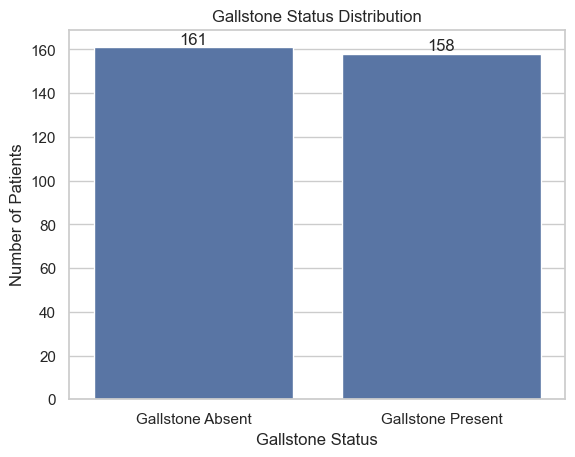
\includegraphics[width=0.8\textwidth]{media/binary_target_distirbution.png} 
    \caption{Distribution of Gallstone Status in the raw dataset.} 
    \label{fig:target-distribution} 
\end{figure} 

The dataset contains 161 participants with gallstones and 158 participants without gallstones. The two classes therefore account for approximately 50.5\% and 49.5\% of the observations, respectively. This indicates that the classification problem is almost perfectly balanced. This is an important characteristic for the subsequent modelling stage. Severe class imbalance is unlikely to be a major source of bias, and resampling techniques such as oversampling or undersampling are not immediately required. Nevertheless, stratified data partitioning will be used when dividing the observations into training and testing sets to preserve the approximately equal class proportions. Model evaluation will also consider sensitivity, specificity, F1-score and ROC-AUC rather than accuracy alone.

\subsubsection{Distribution of Continuous Features}
\label{sec:cont_distribution}

\begin{figure}[H]
    \centering
    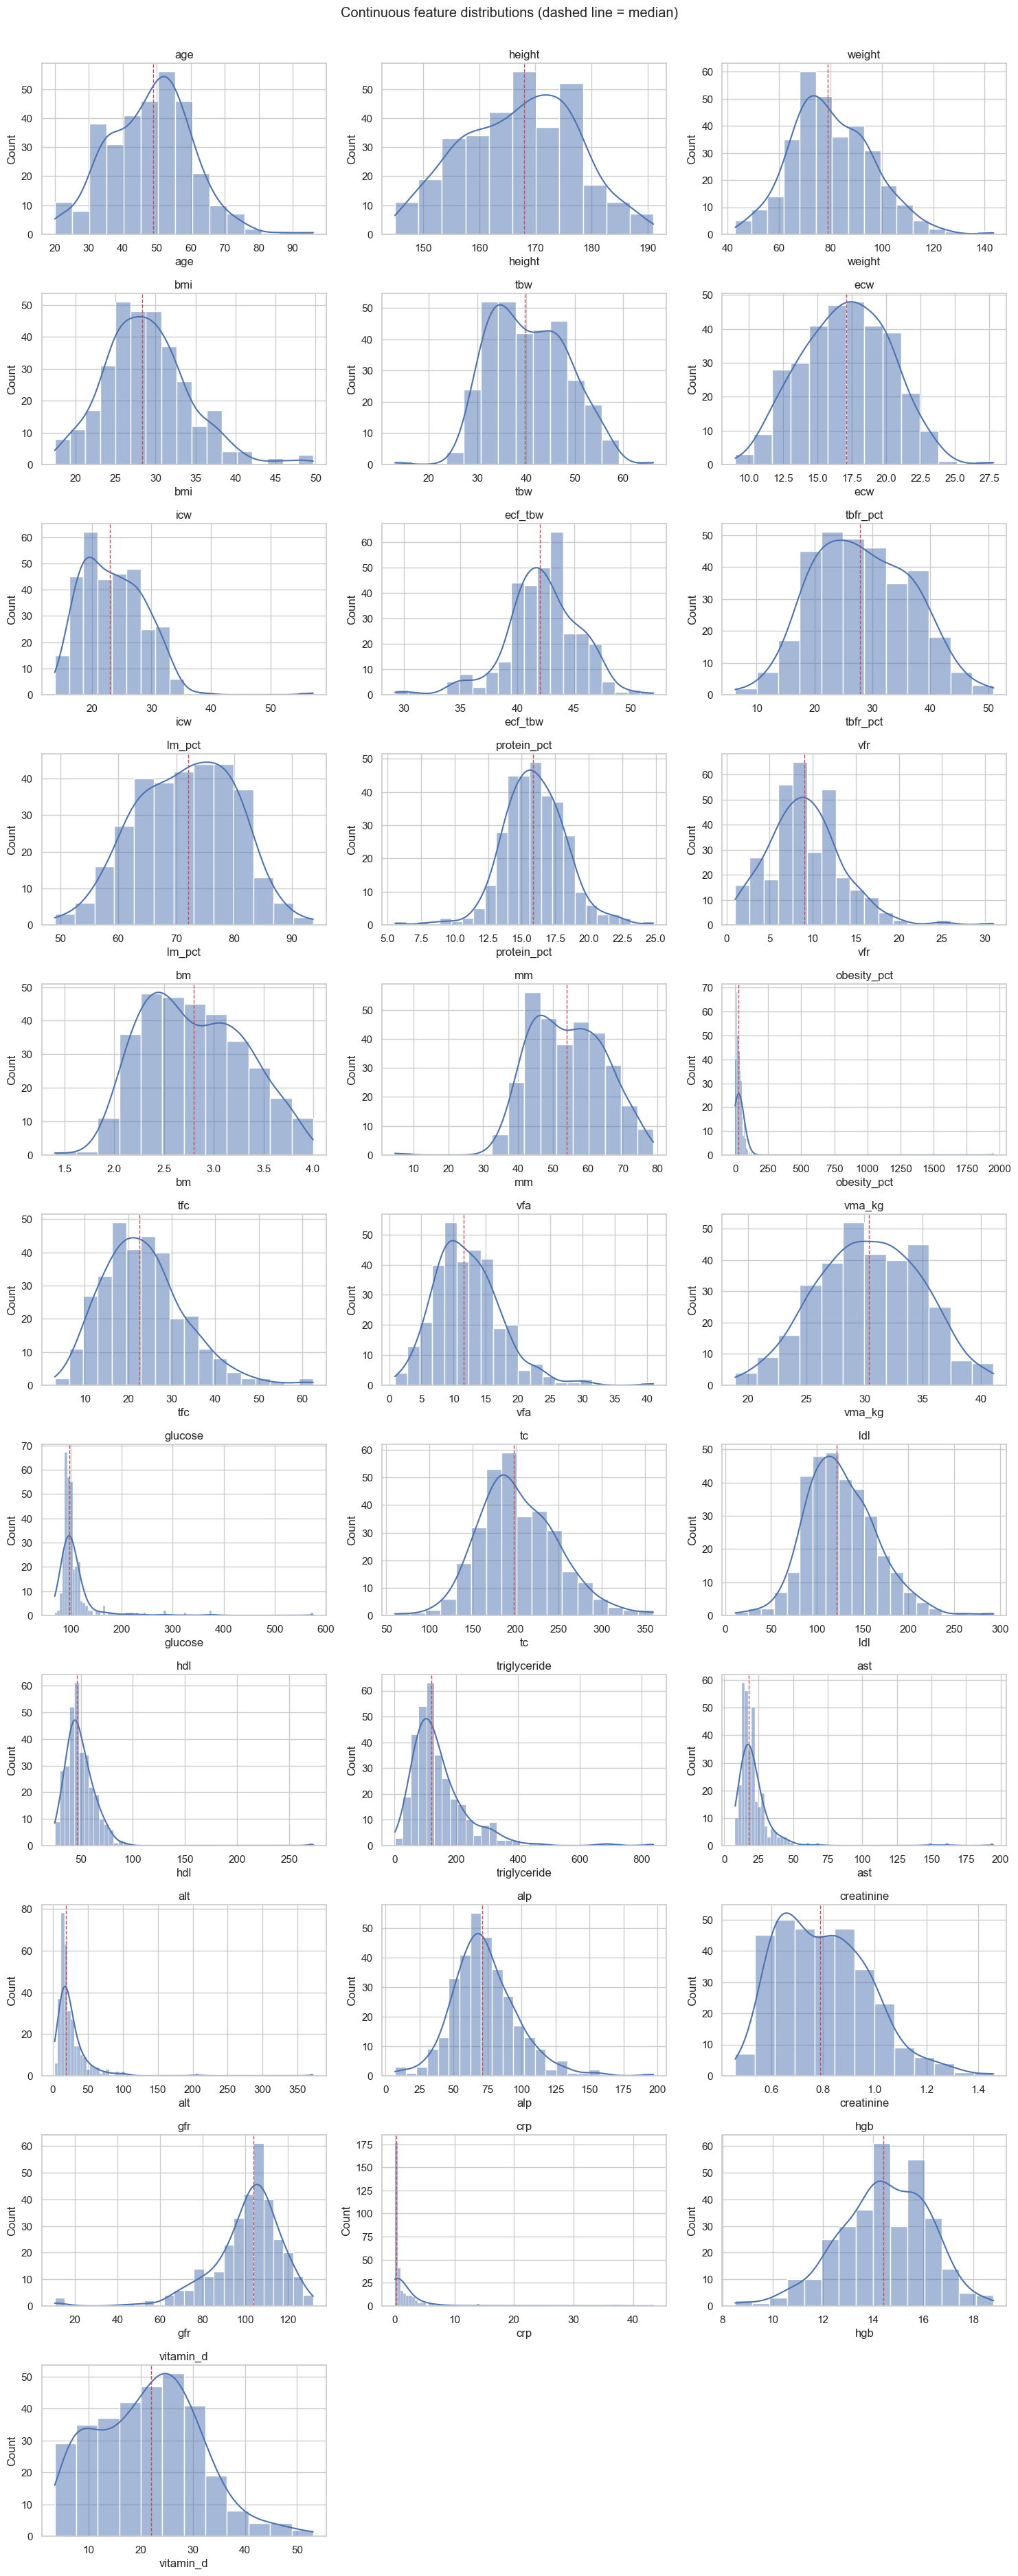
\includegraphics[
        width=\linewidth,
        height=0.75\textheight
    ]{media/Continous_Distribution.png}
    \caption{Distribution of continuous variables in the raw Gallstone dataset.
    The dashed vertical line represents the median.}
    \label{fig:cont-dis}
\end{figure}

Figure~\ref{fig:cont-dis} presents the distributions of the continuous variables before any transformation or outlier treatment. The plots show considerable variation in distributional shape across the clinical and body-composition measurements.

Several variables, including age, height, BMI, extracellular water (ECW), lean mass, creatinine, haemoglobin, and visceral muscle area, display relatively smooth and approximately unimodal distributions. In contrast, variables such as glucose, triglyceride, AST, ALT, CRP, visceral fat rating (VFR), visceral fat area (VFA), and total fat content (TFC) show noticeable right-skewness, with most observations concentrated at lower values and a small number of substantially larger measurements.

The distributions also reveal several extreme observations, particularly in metabolic and laboratory variables. These values require further assessment during the data-quality stage to determine whether they represent valid clinical measurements or potential data errors. They will not be removed automatically, as unusual values may contain clinically meaningful information relevant to gallstone risk.

Overall, this exploration indicates that the predictors differ substantially in both scale and distribution. Consequently, standardisation and possible transformations of strongly skewed variables will be considered during data preparation, depending on the modelling technique used. The next stage of the analysis compares these predictors with \textit{Gallstone Status} to identify variables that may provide useful discriminatory information for the classification models.

\subsubsection{Distribution of categorical features and Association with Gallstone Status}
\label{subsubsec:categorical-distribution}

The categorical predictors were examined by comparing both the class counts and
the proportion of participants with gallstones within each category. This
provides an initial indication of whether particular categorical variables may
contain useful discriminatory information for the prediction task.

\begin{figure}[H]
    \centering
    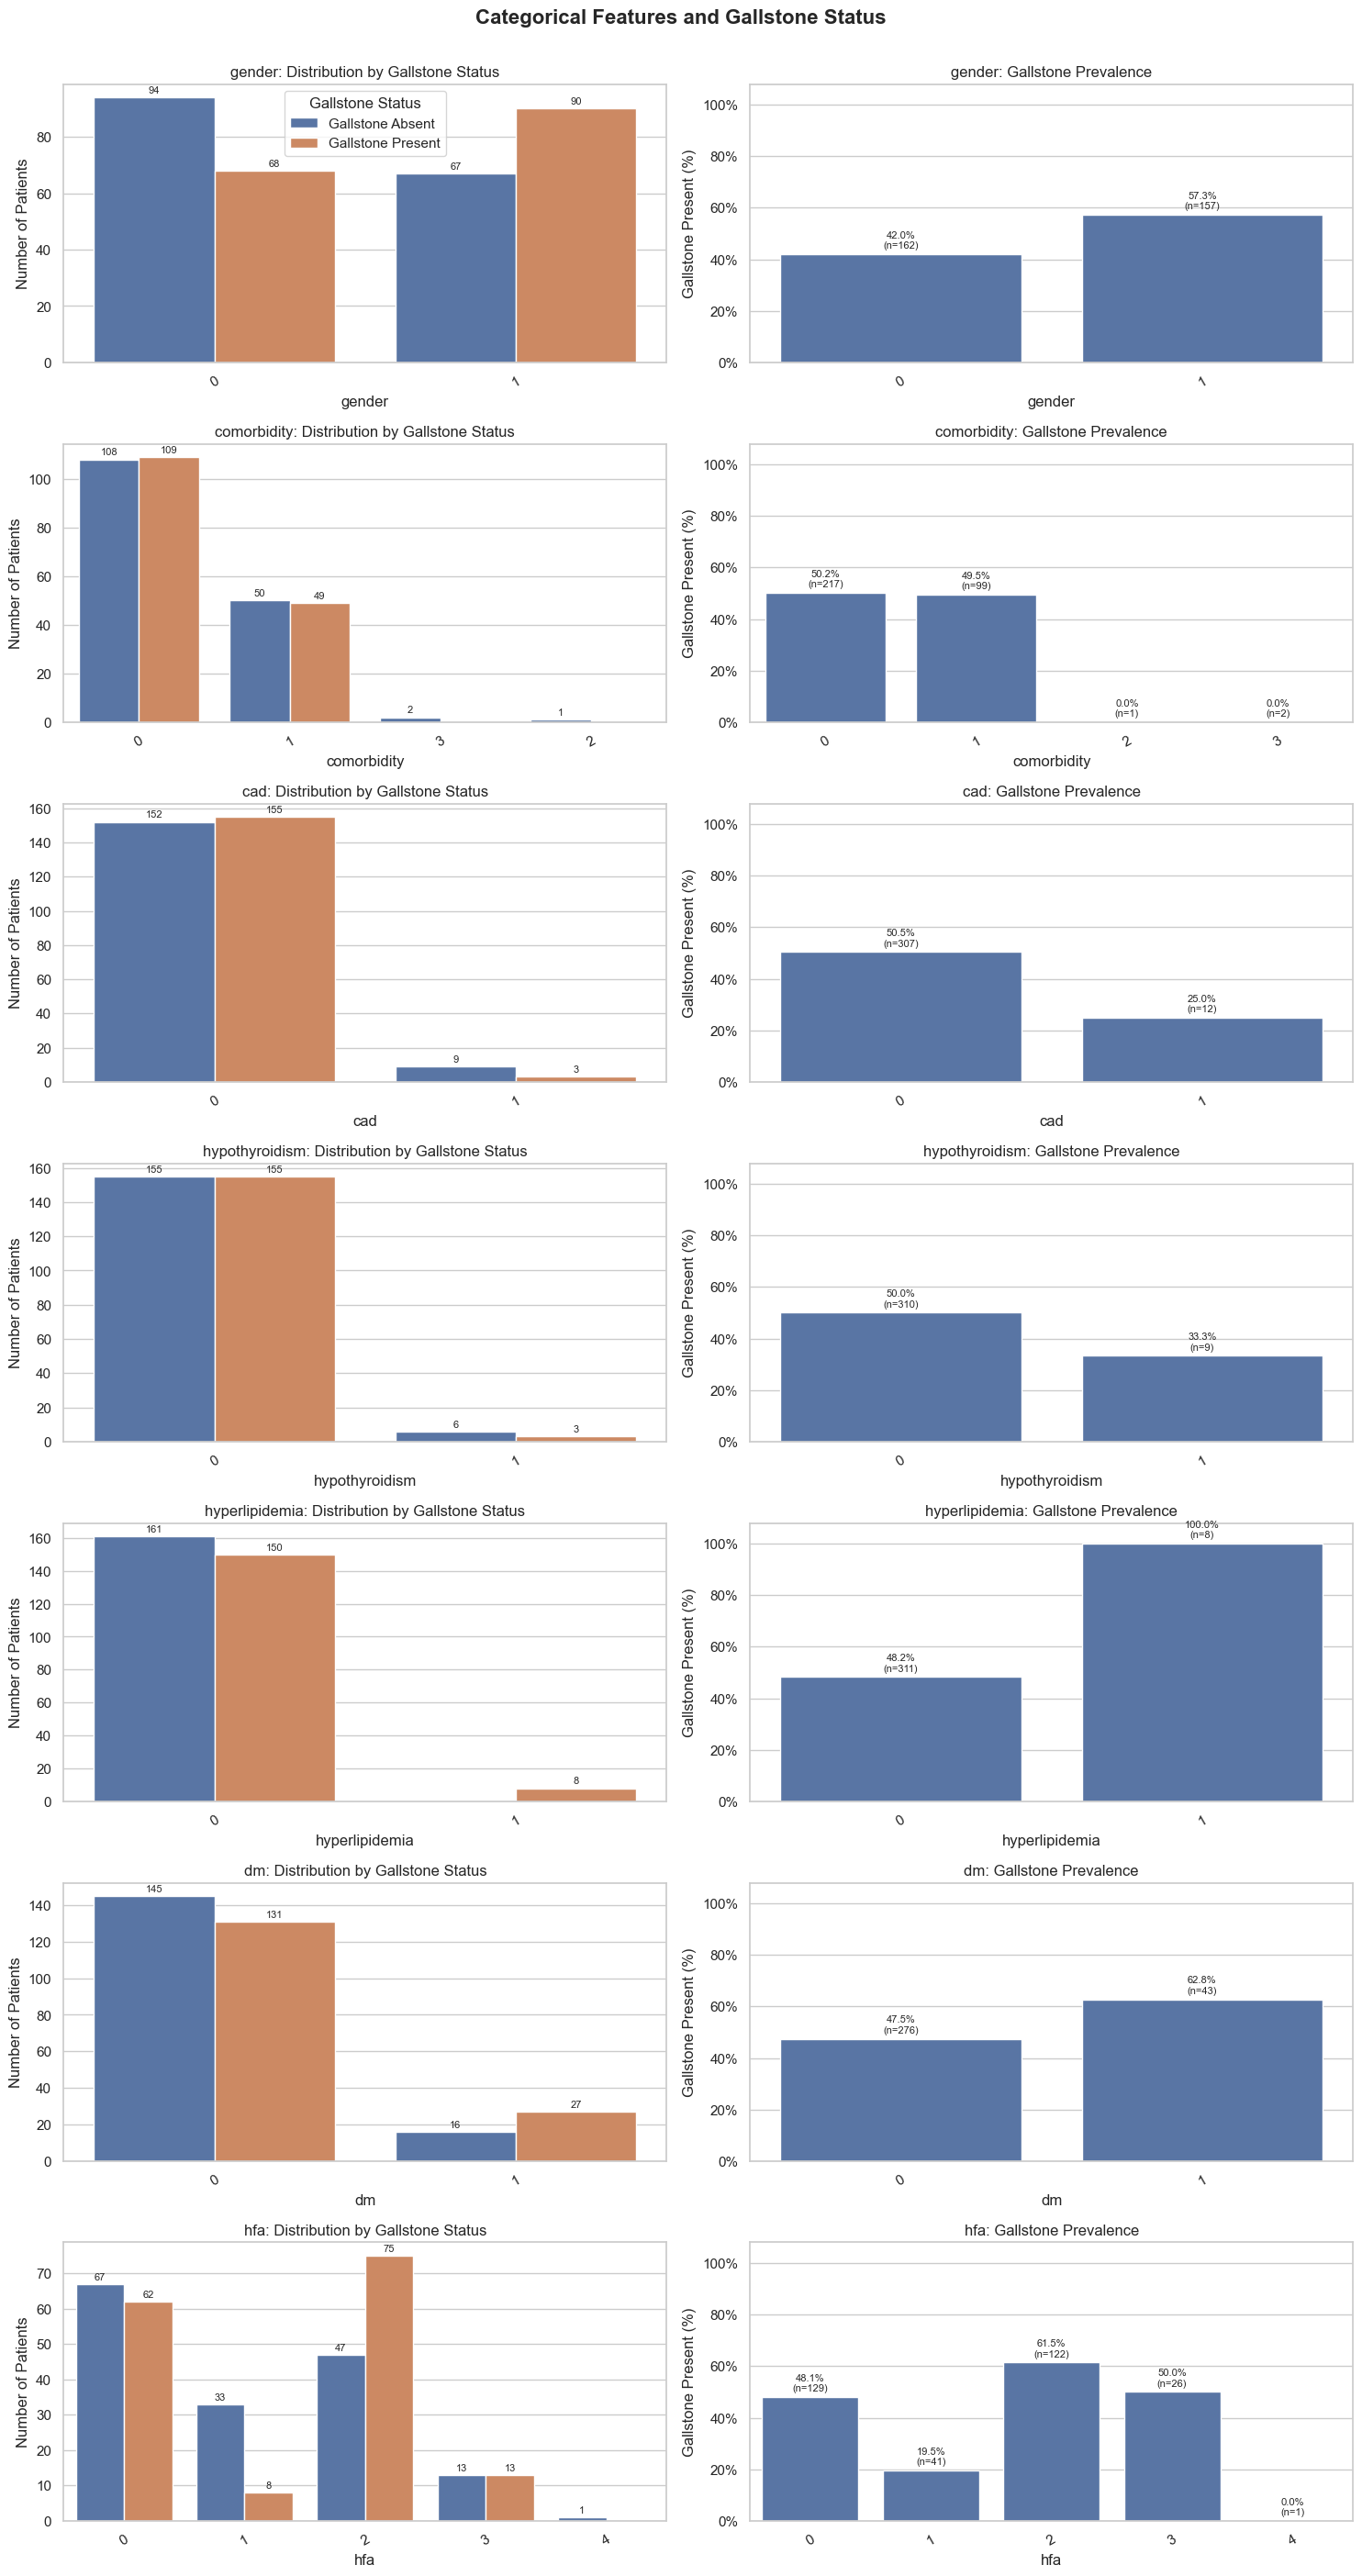
\includegraphics[
        width=0.7\linewidth,
        keepaspectratio
    ]{media/category_distribution.png}
    \caption{Distribution of categorical predictors by Gallstone Status and the
    corresponding gallstone prevalence within each category.}
    \label{fig:categorical-distribution}
\end{figure}

Figure~\ref{fig:categorical-distribution} suggests that the predictive signal
varies considerably across the categorical variables. Gender shows a moderate
difference between categories: the gallstone prevalence is approximately
42.0\% for category 0 and 57.3\% for category 1, indicating that gender may
provide some discriminatory information.

Diabetes mellitus (\texttt{dm}) also shows a potentially useful difference.
Gallstone prevalence is approximately 47.5\% among participants in category 0
compared with 62.8\% in category 1. A similar pattern is visible for
\texttt{hfa}, where prevalence varies across categories, most notably between
category 1 (19.5\%) and category 2 (61.5\%). This suggests that these variables
may contribute information useful for separating the two outcome classes.

In contrast, \texttt{comorbidity} shows little separation in the two major
categories, with gallstone prevalence close to 50\% in both. This indicates
limited univariate discriminatory value for this variable. \texttt{cad} and
\texttt{hypothyroidism} also show lower prevalence among category 1 than
category 0, although the number of observations in their positive categories is
small.

The strongest apparent difference is observed for \texttt{hyperlipidemia},
where all eight participants in category 1 have gallstones. However, this result
should be interpreted cautiously because the category contains very few
observations. Similar caution is required for rare levels of
\texttt{comorbidity} and \texttt{hfa}, where prevalence estimates are based on
only one or two participants and are therefore highly unstable.

Overall, the categorical EDA provides evidence of some class-related signal,
particularly for gender, diabetes mellitus, and selected HFA categories.
However, no single categorical predictor provides a sufficiently strong or
stable separation between participants with and without gallstones. The results
therefore support retaining these variables for multivariable modelling, where
their combined effects and interactions with continuous clinical and
body-composition measurements can be evaluated.


\subsubsection{Correlation Analysis}
\label{subsubsec:correlation}

Figure~\ref{fig:spearman-correlation} presents the Spearman correlationmatrix for the dataset. Spearman correlation was selected because several
continuous variables are skewed and contain extreme observations.

\begin{figure}[H]
    \centering
    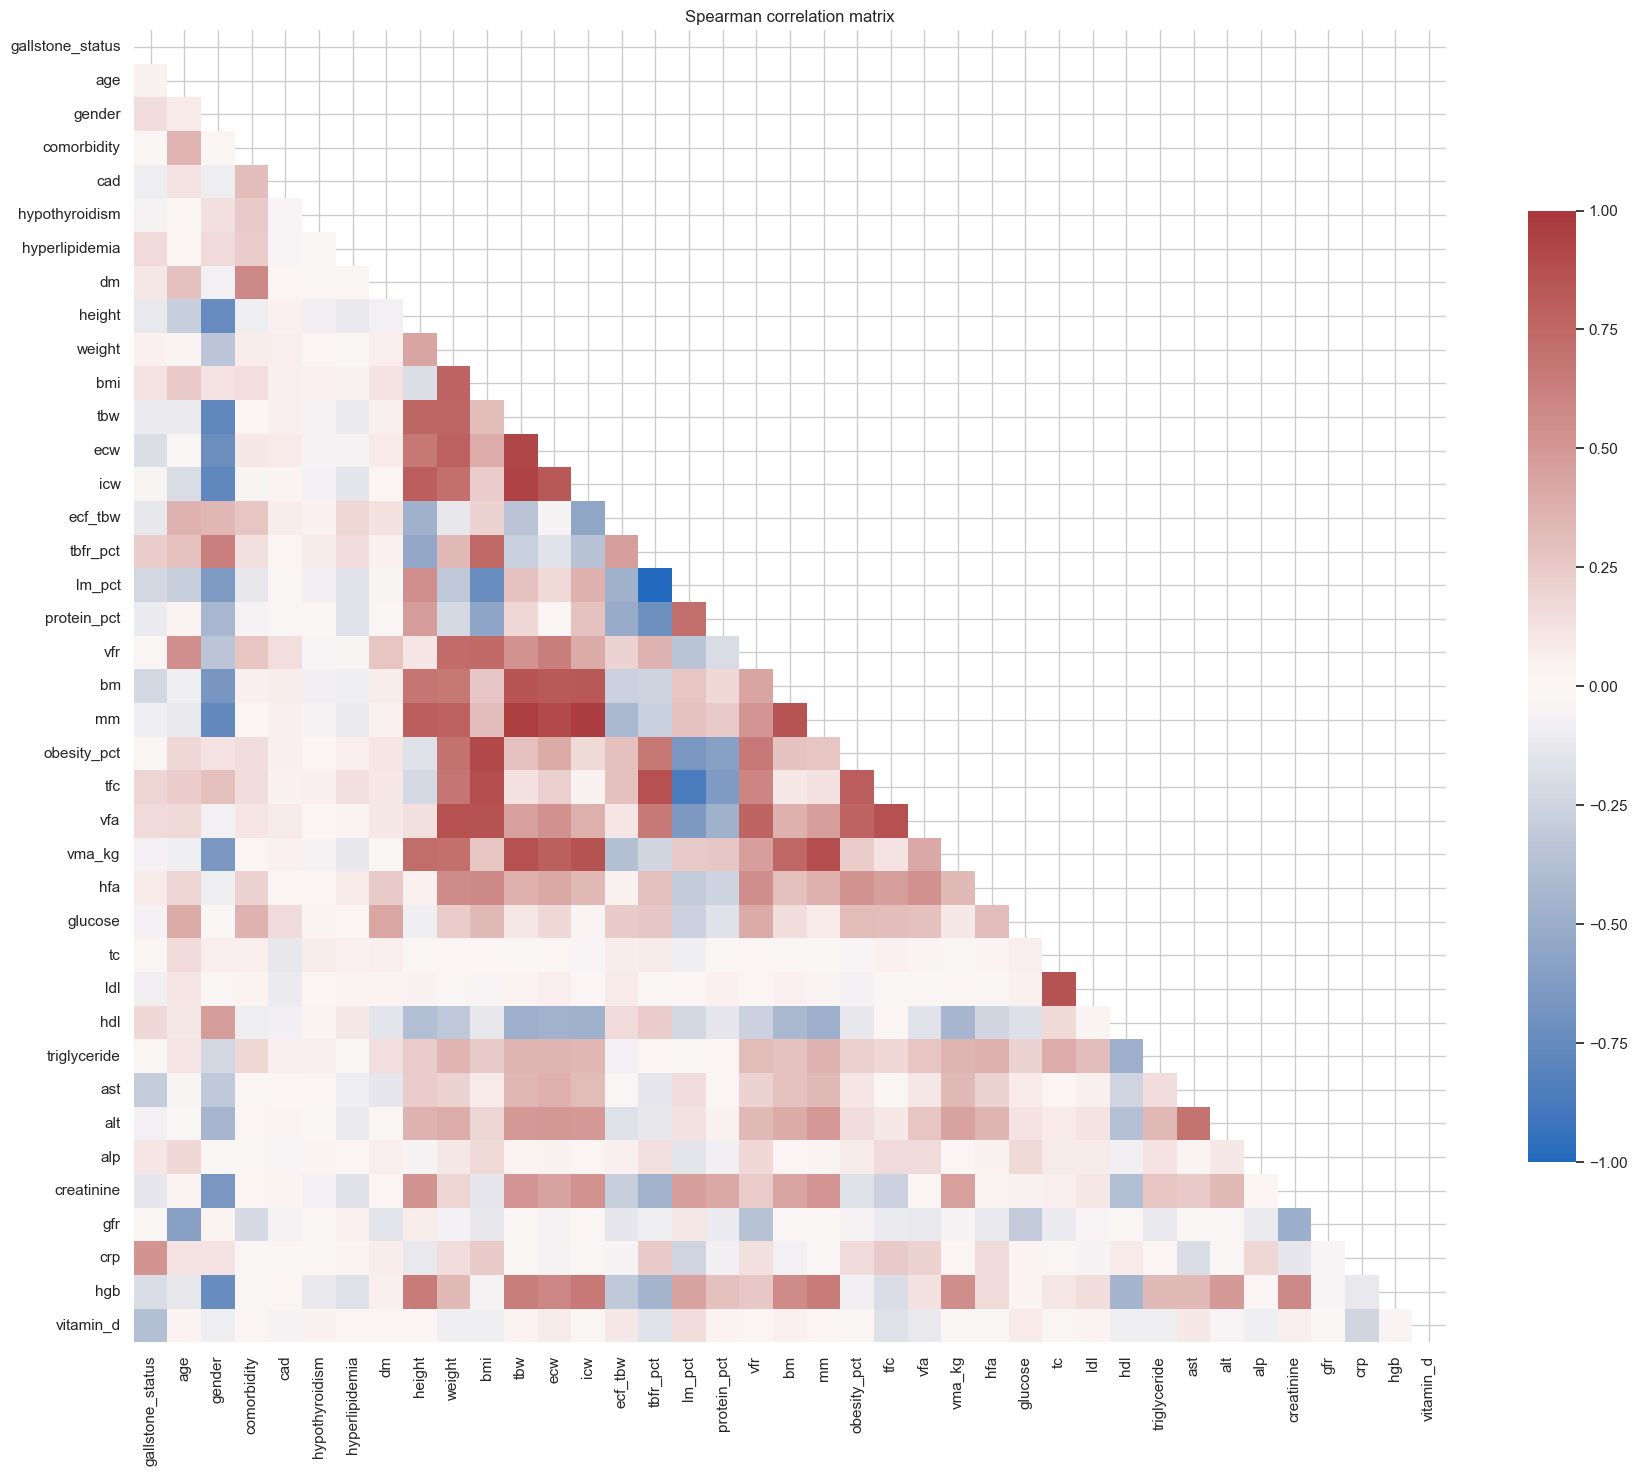
\includegraphics[width=0.75\textwidth]{media/correlation.png}
    \caption{Spearman correlation matrix for the Gallstone dataset visualization.}
    \label{fig:spearman-correlation}
\end{figure}

The matrix shows several groups of strongly related predictors. In particular, body-composition variables such as weight, BMI, TBW, ECW, ICW, muscle mass, body-fat measures, and visceral-fat measures show substantial correlation. Laboratory variables also contain related groups, including
TC-LDL, AST-ALT, and the inverse relationship between creatinine and GFR. These patterns indicate potential redundancy and multicollinearity among some predictors.

In contrast, individual correlations with \textit{Gallstone Status} are generally weaker. This suggests that gallstone status is unlikely to be explained by a single predictor and supports the use of multivariable classification models that combine demographic, body-composition, and
laboratory information.

These findings will guide the data-preparation stage. Highly correlated variables will be reviewed during feature selection, particularly for logistic regression, while tree-based models will also be considered because they are less sensitive to multicollinearity.


\subsubsection{Structure Among Body-Composition Variables} 

Some body-composition variables, including total body water (TBW), bone mass (BM), and muscle mass (MM), appear to have broader or mildly multi-peaked distributions. This may indicate underlying differences between participant subgroups, for example differences in sex, body size, or body composition. At this stage, however, the univariate plots alone are insufficient to determine the cause. Furthermore, several predictors measure related physiological concepts. For example, BMI, TBFR, TFC, VFR and VFA all contain information relating to body fat or adiposity, while TBW, ECW and ICW describe different components of body watxer. Consequently, correlation analysis will be conducted in the next stage to determine whether some predictors contain highly overlapping information. Highly correlated variables will be reviewed before modelling to reduce unnecessary redundancy and potential multicollinearity, particularly for regression-based classifiers.


Overall, the EDA provides the foundation for the next data-preparation phase by identifying class balance, distributional characteristics, outliers, potentially informative predictors, and redundant variables. These findings will subsequently guide preprocessing, feature selection, model selection, and evaluation.

\subsection{Data Quality}
Data quality was assessed before any transformation or model development to ensure that errors in the raw data would not be carried into the predictive models. The verification focused on missing values, duplicate records, categorical coding, numerical ranges, and potential outliers. 

\subsubsection{Missing Values and Completeness} 
The dataset documentation reports no missing values, and this was confirmed during the initial inspection of the dataset. Therefore, no imputation was required at this stage. Nevertheless, missing-value checks will remain part of the preprocessing workflow to ensure that any values introduced during transformation or partitioning are detected before modelling.


\subsubsection{Potential Outliers and Data Quality Issues} 
\label{sec:outliers}

\begin{figure}[H]
    \centering
    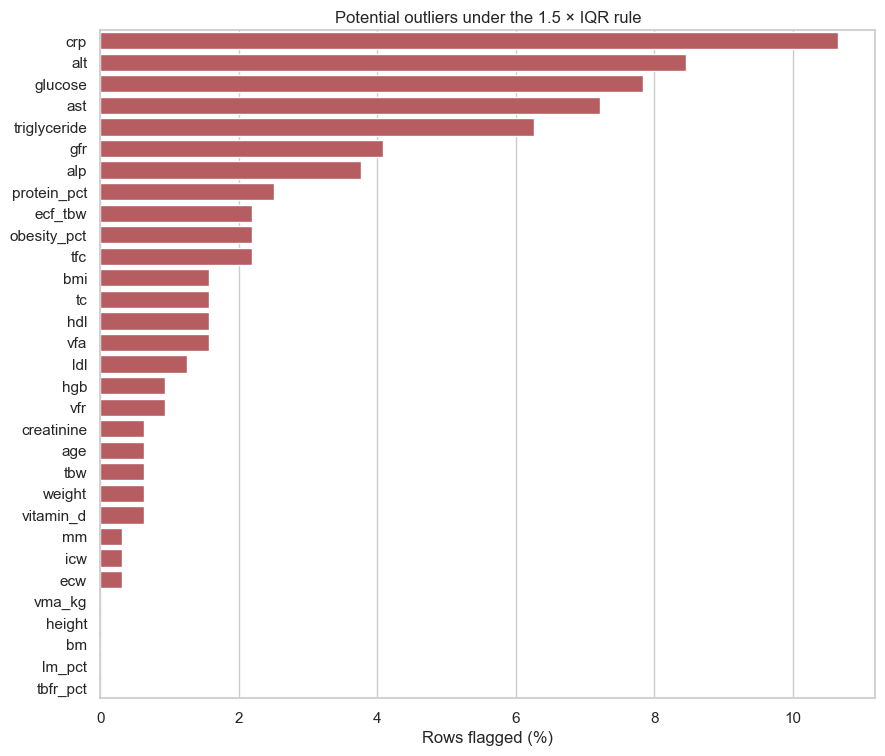
\includegraphics[width=\linewidth]{media/Outlier_Analysis.png}
    \caption{Outlier analysis using the 1.5$\times$IQR method.}
    \label{fig:outlier-analysis}
\end{figure}

Figure~\ref{fig:outlier-analysis} identifies several observations that require further investigation. Most notably, the \textit{Obesity} variable contains an extreme value of approximately 2000, which is substantially larger than the remaining observations. Given the magnitude of this difference, the value should be verified against the original dataset and variable definition to determine whether it represents a valid measurement, a unit inconsistency, or a data-entry error.

Potential upper-tail outliers are also observed in variables including glucose, HDL, triglyceride, AST, ALT, CRP, and intracellular water (ICW). However, observations identified by the 1.5$\times$IQR rule should not automatically be treated as erroneous, particularly in clinical data where extreme measurements may represent genuine patient conditions. Therefore, these observations will be reviewed during data preparation before any correction, transformation, or removal is applied.

Valid extreme observations will be retained where appropriate to preserve clinically meaningful variation in the dataset. Only values supported by evidence of coding, measurement, or data-entry errors will be considered for correction or exclusion. This approach reduces the risk of removing informative clinical cases and introducing bias into subsequent predictive models.


\subsubsection{Dimensionality Reduction Visualisation and Data Understanding}
\label{subsubsec:dimensionality_reduction}

Dimensionality-reduction techniques were used to obtain a more compact view of
the relationships among the continuous measurements and to assess whether
participants with and without gallstones exhibit distinct multivariate patterns.
Two complementary approaches were considered: Principal Component Analysis
(PCA) and t-distributed Stochastic Neighbor Embedding (t-SNE). PCA provides a
linear representation of the dominant sources of variance in the data, whereas
t-SNE is a nonlinear technique designed to preserve local neighbourhood
relationships in a low-dimensional representation
\parencite{vandermaaten2008tsne}.

\paragraph{Principal Component Analysis}

PCA was first applied to the continuous measurements to examine the main
directions of variation in the dataset. The first principal component (PC1)
explained 27.7\% of the total variance, while the second principal component
(PC2) explained a further 20.0\%. Together, the first two components therefore
accounted for approximately 47.7\% of the variance in the continuous feature
space.

\begin{figure}[H]
    \centering
    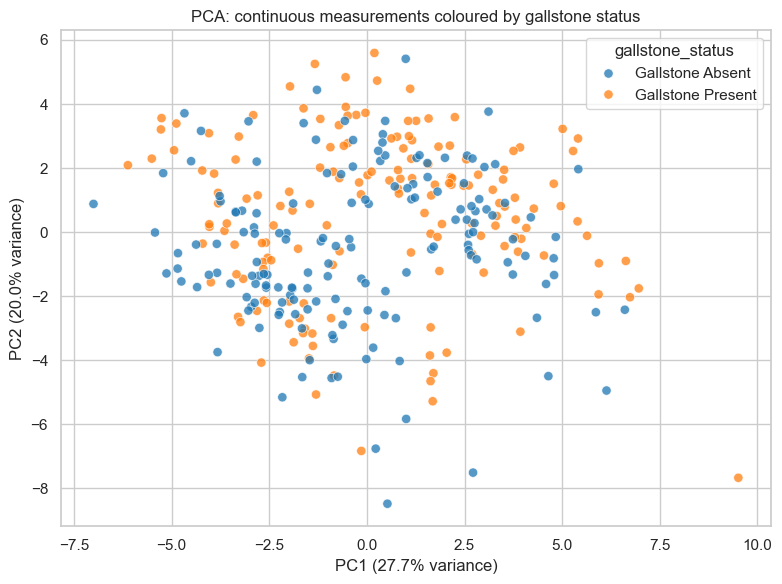
\includegraphics[
        width=0.76\linewidth,
        keepaspectratio
    ]{media/PCA.png}
    \caption{Two-dimensional PCA projection of the continuous measurements,
    coloured by Gallstone Status. PC1 and PC2 explain 27.7\% and 20.0\% of the
    total variance, respectively.}
    \label{fig:pca_projection}
\end{figure}

As shown in Figure~\ref{fig:pca_projection}, observations from the
\textit{Gallstone Present} and \textit{Gallstone Absent} groups overlap
substantially in the first two principal components. No distinct linear
separation between the two outcome groups is apparent. This indicates that the
largest sources of variation in the continuous measurements are not themselves
equivalent to the variation that separates gallstone status.

Nevertheless, the projection reveals meaningful structure within the
measurements. Participants are distributed across several regions of the PCA
space, suggesting heterogeneity in body-composition, anthropometric, and related
clinical characteristics. A small number of observations also lie relatively
far from the central concentration of the data. These observations are
consistent with the unusual or extreme measurements identified during the
earlier univariate exploration and were retained for further investigation
rather than being removed solely on the basis of their position in the PCA
projection.

To understand which variables contribute most strongly to the two principal
components, the corresponding PCA loadings were also examined.

\begin{figure}[H]
    \centering
    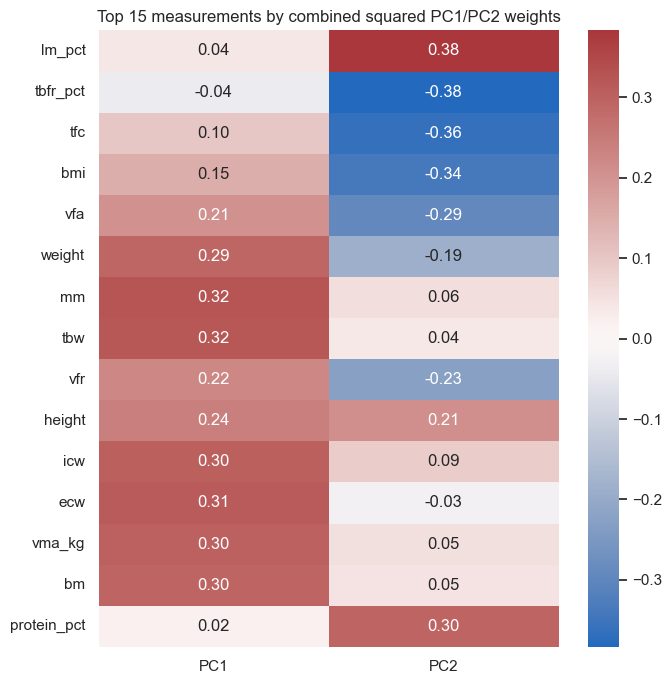
\includegraphics[
        width=0.62\linewidth,
        keepaspectratio
    ]{media/PCA_weight_measurement.png}
    \caption{Loadings of the 15 continuous measurements with the largest
    combined squared contributions to PC1 and PC2. Positive and negative values
    indicate the direction of association with each principal component.}
    \label{fig:pca_loadings}
\end{figure}

Figure~\ref{fig:pca_loadings} shows that PC1 is influenced primarily by several
body-size and body-composition measurements. Muscle mass (\texttt{mm}),
total body water (\texttt{tbw}), extracellular water (\texttt{ecw}),
intracellular water (\texttt{icw}), visceral muscle area
(\texttt{vma\_kg}), bone mass (\texttt{bm}), weight, and height all have
positive loadings on PC1. This suggests that PC1 broadly represents variation
associated with overall body size and lean/body-composition characteristics.

PC2 captures a different contrast. Lean-mass percentage
(\texttt{lm\_pct}) and protein percentage (\texttt{protein\_pct}) have strong
positive loadings, whereas total body-fat percentage (\texttt{tbfr\_pct}),
total fat content (\texttt{tfc}), BMI, visceral fat area (\texttt{vfa}), and
visceral fat rating (\texttt{vfr}) have negative loadings. PC2 can therefore be
interpreted as reflecting a contrast between lean-body composition and
fat-related measurements. These loading patterns provide additional insight into
the correlations among the original measurements and help explain the structure
observed in the PCA projection.

\paragraph{t-SNE Visualisation}

Because PCA represents only linear combinations of the original variables, a
nonlinear t-SNE analysis was additionally performed to examine whether local
neighbourhood structures could reveal patterns that were not visible in the PCA
projection. Multiple perplexity values were evaluated rather than relying on a
single t-SNE configuration.

\begin{figure}[H]
    \centering
    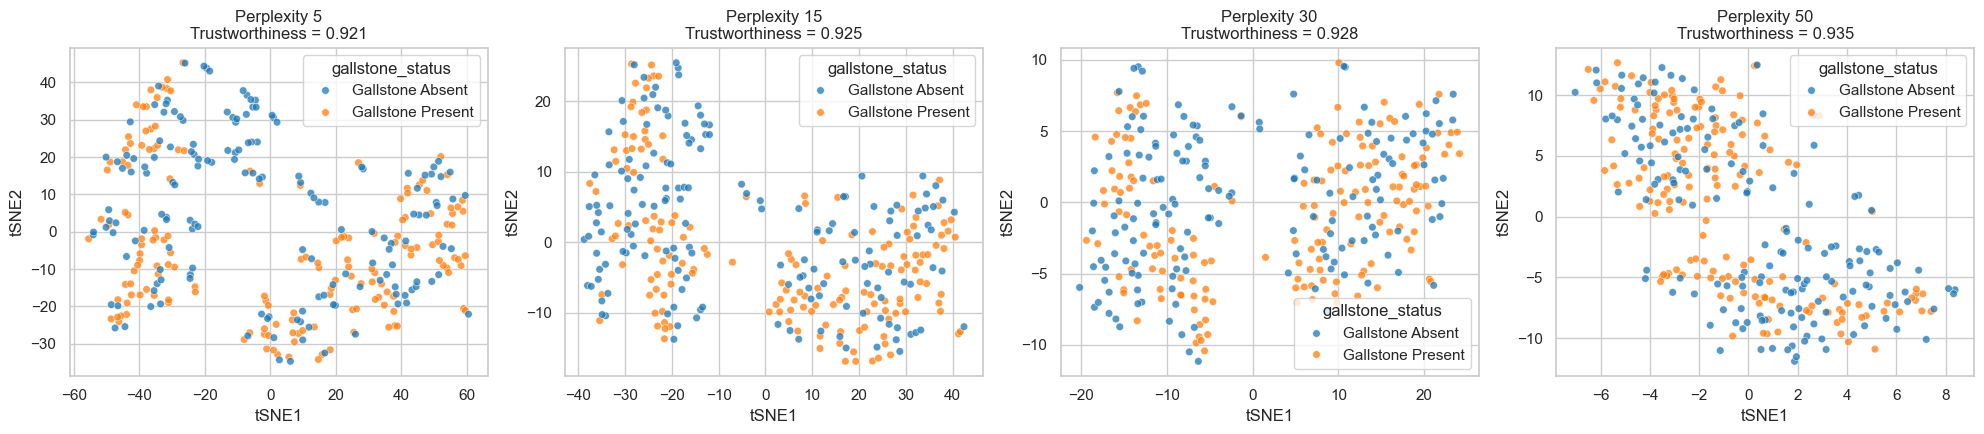
\includegraphics[
        width=\linewidth,
        keepaspectratio
    ]{media/TSNE_visualization.png}
    \caption{Two-dimensional t-SNE projections of the continuous measurements
    using perplexity values of 5, 15, 30, and 50. Points are coloured according
    to Gallstone Status. Trustworthiness scores are reported for each
    configuration.}
    \label{fig:tsne}
\end{figure}

Figure~\ref{fig:tsne} shows that the overall appearance of the t-SNE
representation changes as the perplexity parameter increases. Lower perplexity
values, particularly 5, emphasise very local neighbourhoods and produce a more
fragmented representation. At larger perplexities, the observations form
broader and more coherent structures.

The trustworthiness score increased from 0.921 at perplexity 5 to 0.935 at
perplexity 50, indicating that the higher-perplexity representations preserved
the original local neighbourhood relationships slightly more effectively.
However, the purpose of this metric is to assess preservation of neighbourhood
structure rather than separation of the target classes.

Across all perplexity settings, participants with and without gallstones remain
substantially intermixed. Although some local regions contain a greater
concentration of one class than the other, there is no stable class-specific
cluster or simple visual boundary that consistently separates
\textit{Gallstone Present} from \textit{Gallstone Absent}. The same general
conclusion is therefore observed in both the linear PCA representation and the
nonlinear t-SNE representations.


These findings suggest that gallstone status is unlikely to be explained by a
single dominant measurement or by a simple low-dimensional boundary. Instead,
the predictive information may be distributed across several demographic,
body-composition, metabolic, and biochemical variables and may involve
interactions or nonlinear relationships among them. This observation motivates
the subsequent comparison of multivariable classification models.

Importantly, both PCA and t-SNE were used here as exploratory tools for data
understanding rather than as measures of predictive performance. Visual overlap
between the classes does not imply that the target is unpredictable, since
discriminative information may exist in dimensions that are not represented by
the first two principal components or by the two-dimensional t-SNE embedding.
Model performance is therefore assessed separately using the validation and test
partitions.